% vim:ft=tex
\section{Prediction on Daily Basis}\label{sec:daily}
\subsection{Data Profiling Part II}\label{dp2}
As already indicated in Data Profiling Part 1 in chapter \ref{dp1}, the next step is to display the use of the routes at
different times between the individual bicycle stations on a map. Since the Python package
"folium" uses leaflet maps based on Javascript \cite{RN5}, the plotting of the routes on an hourly level is
not performant, because too many polylines have to be drawn and the map can no longer be
efficiently displayed in the browser. Therefore only the top 10\% most used routes were plotted on
the folium map. Another restriction was the aggregated granularity on a daily base. This means
that the plotted map always showed the route usage for day x. With the folium plugin
\glqq TimestampedGeoJson\grqq time series data can be plotted in JSON format. An excerpt from the
script \glqq Cycleusage \& Cycleroutes [allStations].ipynb\grqq shows the corresponding function call:
\begin{figure}[H]
\hspace{-1.6cm}
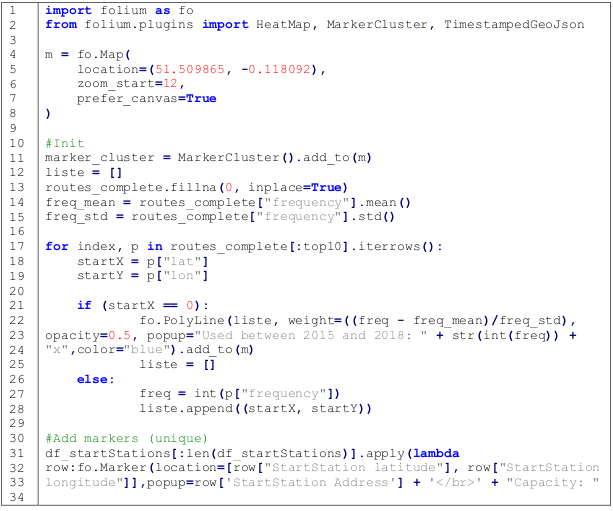
\includegraphics[width=1.2\textwidth]{img/listing1}\label{fig:listing1}
%\captionof{figure}{Result of \acs{mlp} with MinMaxScaler}\label{fig:listing1}
\end{figure}
\begin{figure}[H]
\hspace{-1.6cm}
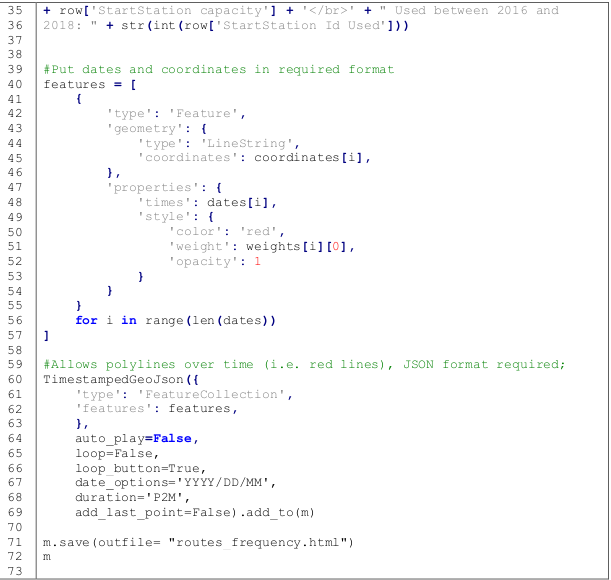
\includegraphics[width=1.2\textwidth]{img/listing2}\label{fig:listing2}
\captionof{figure}{Route usage over time plot}\label{fig:listing2}
\end{figure}
As the code from figure \ref{fig:listing2} shows, the polylines on the map have been added iteratively. The
weight parameter can be used to determine the thickness of the polyline. Since these should look
as dynamic as possible on the map, the weight has been standardized. The fixed stations were
initially added, but no duplicate stations were plotted. A disadvantage of the plugin is that it needs
the data in a JSON format. Therefore the coordinates for the single points of a polyline as well as
the time series data had to be converted into a compatible format. As can be seen from the Python
code, the coordinates must be given the type \glqq LineString\grqq.  A LineString is defined as a sequence
of uniquely assignable points. In this case, the longitude and latitude previously requested using
the Graphhopper API on our Graphhopper server were sufficient. It is important that the parameter \glqq date\_options\grqq in \glqq TimestampedGeoJson\grqq corresponds exactly to the date format as in the nested
list dates, otherwise the time slider function on the map will not work properly.
Applied to the bicycle data the following picture results for the time 26.06.2016:
\begin{figure}[H]
\hspace{-1.6cm}
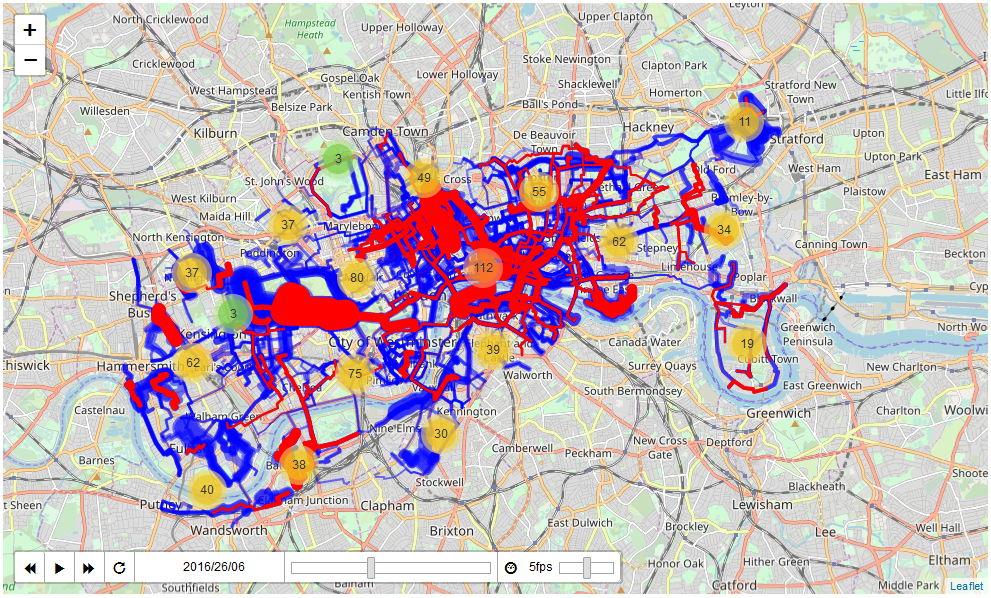
\includegraphics[width=1.2\textwidth]{img/figure4_folium_plot1}\label{fig:figure4_folium_plot1}
\captionof{figure}{Used bicycle routes over time plot}\label{fig:figure4_folium_plot1}
\end{figure}
From figure \ref{fig:figure4_folium_plot1} it can be seen that on this day there was a moderate use of Santander Bicycles in
inner London. Especially the hubs such as Kings Cross or Hyde Park were obviously used very
often with Santander Bicycles on this spring day. Furthermore, the map with the thickness of the
polylines shows how often this route was used in relation to the total use of all routes. The red
colored routes from figure \ref{fig:figure4_folium_plot1} are the actually used routes on this particular day, while the blue
routes are the \glqq inactive\grqq ones. The bubbles with the numbers represent the respective rental
stations. These have only been aggregated to provide a clearer representation. If the map is
zoomed in (figure \ref{fig:figure4_folium_plot1}), the granularity is refined and the markers of the individual rental station
locations are displayed. The color of these bubbles correlates with the number of aggregated
stations in the vicinity. This method also has the advantage that it is easy to see where most rental
stations are located. In fact, with 112 stations (see figure \ref{fig:figure4_folium_plot1}), the inner districts connected by the
Waterloo Bridge and the London Blackfriars Bridge form the centre of most stations which are
close by. It should be noted, however, that new rental stations are constantly being added (even
given up again!), and a new data extract could result in a different picture. Therefore this assumption is valid for the selected date from figure \ref{fig:figure4_folium_plot1}, but not for today or in two years. A useful
feature that comes along with the folium plugin is the automatic data display sequence \cite{RN5}. When
someone clicks on the \glqq Play\grqq button from figure \ref{fig:figure4_folium_plot1}, all time series data is automatically run through.
The speed can be adjusted with the \glqq fps\grqq slider.
To give a counterexample, the following map shows the use of the routes on a winter’s day:
\begin{figure}[H]
\hspace{-1.6cm}
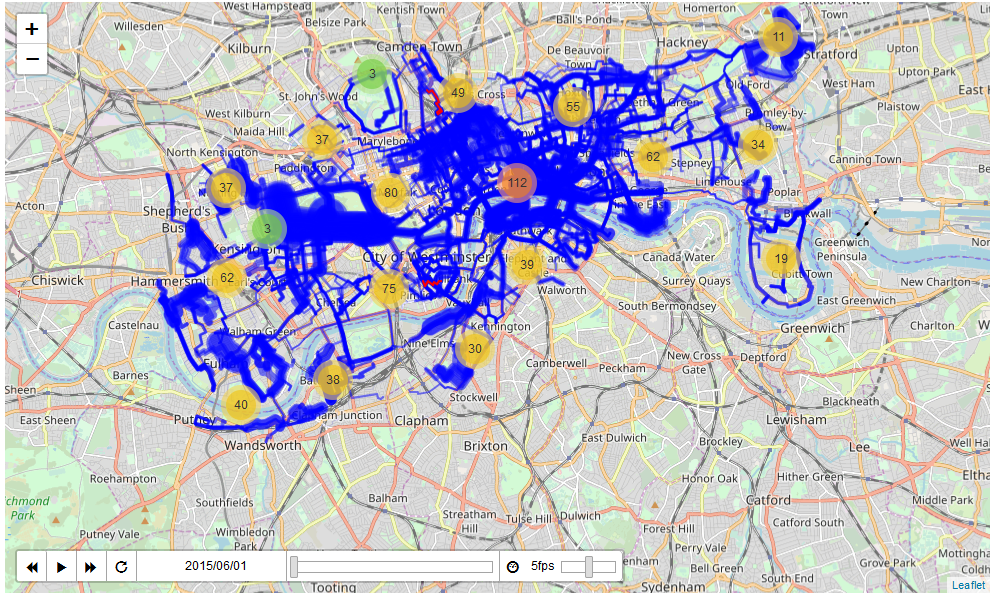
\includegraphics[width=1.2\textwidth]{img/figure5_folium_plot2}\label{fig:figure5_folium_plot2}
\captionof{figure}{Used bicycle routes over time plot}\label{fig:figure5_folium_plot2}
\end{figure}
On 06.01.2015 obviously less bicycles were rented than in figure \ref{fig:figure4_folium_plot1}. This is due to the fact that at
this time it was winter and on the other hand there were only 315 Santander bicycle rental stations
all over London \cite{RN6}. In the course of time, new stations were added again and again, resulting in
a network which is monitored and managed by the local government and administrated by TfL.
The interactive map is also available on the \href{http://i-hadoop-01.informatik.hs-ulm.de/routes_frequency.html}{Hadoop Cluster}.
Overall, it can be observed that the usage of the rental stations has risen sharply on average over
the last four years. This can be explained by the expansion of the network but also by the increased
environmental awareness of the citizens. It is to be expected that further stations will be connected
in the future, so that ideally there will be one rental station at each crossroad in the town.
\subsection{Feature Engineering Kings Cross}\label{king}
Next, the features for the most frequently used station (Kings Cross) were prepared and
aggregated on a daily basis. In addition, these features have been extended by more like
\emph{Holidays, Weekdays, Months, Seasons} and weather data. This enrichment of the features
should help to achieve a higher accuracy of the learning model. For the weather data the weather
API \glqq Dark Sky\grqq was used. Like every available weather API the free use is limited. In the case of
Dark Sky a maximum of 1000 API request calls per day can be executed with one key \cite{RN7}.
However, this limitation can be bypassed if multiple accounts are used. Since each account has
a key, the keys can be collected and thus in fact significantly more requests can be executed.
However, this cannot be applied to the existing data sets of the bicycle data, since the daily
aggregated data of Kings Cross alone has already 376625 rows. Therefore a \glqq dates\grqq file was
created, which contains all days from 04.01.2015 - 14.04.2019 and thus covers all possible date
values of the rental station data. This has the advantage that now only 1562 API requests are
necessary and two keys are sufficient. The disadvantage of this method is that of course no precise
weather data can be retrieved at every station. Therefore the coordinates for the weather data of
the centroids (51.509865,-0.118092) of London were chosen. Dark Sky API also returns a JSON
file as response, which can be searched for the desired information. The following function from
the script \glqq Cycleusage \& Cycleroutes [allStations].ipynb\grqq shows the corresponding request call:
\begin{figure}[H]
\hspace{-1.6cm}
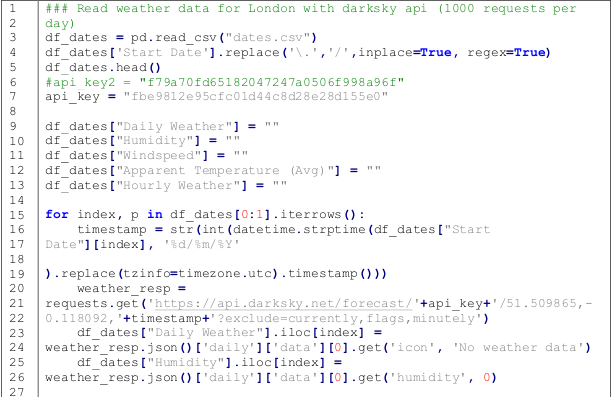
\includegraphics[width=1.2\textwidth]{img/listing3}\label{fig:listing3}
%\captionof{figure}{Result of \acs{mlp} with MinMaxScaler}\label{fig:listing1}
\end{figure}
\begin{figure}[H]
\hspace{-1.6cm}
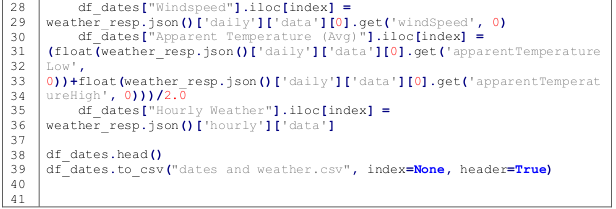
\includegraphics[width=1.2\textwidth]{img/listing4}\label{fig:listing4}
\captionof{figure}{Fetching the weather API with Python}\label{fig:listing4}
\end{figure}
As the code from figure \ref{fig:listing4} clearly shows, the following weather data were considered as relevant:
\glqq Daily Weather, Humidity, Windspeed\grqq and \glqq Apparent Temperature (Avg)\grqq . The feature \glqq Daily
weather\grqq returns a string value, how general the weather was on that particular day (e.g. sunny,
partly-cloudy...). Dark Sky makes this value dependent on the worst condition that occurred on
that day \cite{RN7}. That is, if it snowed for an hour, but the rest of the day was cloudy, \glqq Daily Weather\grqq will still show \glqq snowy\grqq  because this condition is weighted higher.\\\\
In addition to the weather data mentioned above, the hourly weather data of each day was also
queried as JSON lists, as otherwise every hour of each day would have to be queried separately,
which would drastically increase the API calls. A drawback of this variant is that the dates and
weather dataframe has a mixed structure. While the column \glqq hourly weather\grqq is a JSON format,
the other columns have a normal structure. This problem is further addressed in the section \glqq Data
Preparation - Hourly Base\grqq .\\\\
The processed weather data were next merged with the processed cycle usage dataframe. For
the Holidays the Python package \glqq holidays\grqq was used, which returns the corresponding holidays
to a selected location. Similarly, the features \emph{Weekdays, Months} and \emph{Seasons} were be
generated with defined functions and afterwards merged back with the main dataframe.\\\\
Subsequently, the dataframe was supplemented by \glqq past\grqq and\glqq future\grqq data. This should improve
the training of regression models, for example. A kind of \glqq sliding window\grqq was implemented for
the past data. This means that these columns always contain the value of the previous day. With
the future usage data, the daily number of borrowed bikes of the next day was also displayed. The
column \glqq Rented Bikes\grqq (i.e. usage) corresponds to the class variable of interest. This has the
consequence that the first and last day in the dataframe have missing values, because there is no
data for this naturally. The prepared dataframe for Kings Cross on a daily basis looks after the
preparation steps like this:
\begin{figure}[H]
\hspace{-2.8cm}
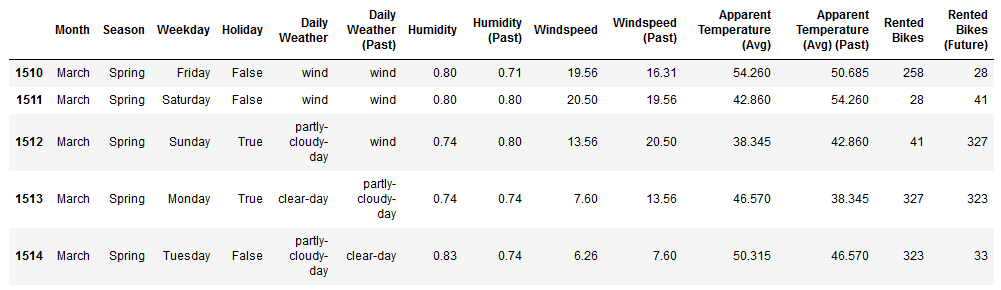
\includegraphics[width=1.4\textwidth]{img/figure6_kings_cross_df}\label{fig:figure6_kings_cross_df}
\captionof{figure}{Prepared data frame of Kings Cross (daily)}\label{fig:figure6_kings_cross_df}
\end{figure}
As one can see from figure \ref{fig:figure6_kings_cross_df}, the past data was only included for the weather data whereas the
future data was only added for the usage of the rental station. The string values were later be
transformed into numerical values since machine learning methods always require number values
instead of string values. Therefore a proper schema was defined, which is described in more detail
in the modelling section.\\\\
With the processed bicycle data from \ref{fig:figure6_kings_cross_df}, machine learning can already be used to predict,
for example, the daily usage of bicycles (i.e. how many bicycles will be borrowed tomorrow starting
from today?). The script \glqq Feature Engineering Kings Cross.ipynb\grqq contains the preparation
functions described above and can be found on our GitHub repository.
\subsection{Data Prediction with MLPRegressor}\label{sec:mlp}
Since we wanted to implement the prediction algorithm in Python we used the library \emph{Scikit Learn} which provides a class \emph{\acf{mlp}} with according functions.
As we wanted to train a non-linear model we decided to use a Multi-layer Perceptron since it can learn a non-linear function approximator for either classification or regression. However  the \acs{mlp} uses backpropagation which is the most widely used algorithm for supervised learning with multi-layered feed-forward networks \cite{riedmiller1993direct}, this algorithm was implemented to train a prediction model for the rental bike usage on a daily base.\\\\
The outcome of of the Data Profiling Part 2, as described in chapter \ref{sec:dp2} served as a basis for the prediction.
As a first implementation we used the following data as an input for the feature matrix: \emph{Month, Weekday, Day, Season, Daily Weather, Daily Weather Past, Humidity, Humidity Past, Windspeed, Windspeed Past, Apparent Temperature (Avg), Apparent Temperature (Avg) Past, Rented Bikes}. Since we assume that weather conditions play an important role in bike usage we decided to add weather data. Another assumption was that on weekdays the frequency will rise, because a lot of people use rented bikes to travel to work. Furthermore we added the number of rentals of today in order to predict the ones of tomorrow. Therefore \emph{Rented Bikes Future} served as our target variable which is to predicted.\\
Since the \acs{mlp} works with data represented as dense and sparse numpy arrays of floating point values, data had to be encoded accordingly beforehand. Therefore we mapped all of the ordinal scaled data like \emph{Month, Weekday, Season, Daily Weather} to numerical data, by implementing a dictionary which assigns numerical values to ordinal data. E. g. For the weekdays we used the following dictionary:
\begin{lstlisting}[language=bash,breaklines=true]
"Weekday": {"Monday": 1, "Tuesday": 2, "Wednesday": 3, "Thursday": 4,"Friday": 5, "Saturday": 6, "Sunday":7 }
\end{lstlisting}
After the encoding we split the data into 80 \% training data and 20\% test data.
Since the \acs{mlp} is sensitive to feature scaling we normalized the data accordingly to the activation function. Since we used the \emph{logistic} activation function which expects values between [0,1] we normalized the feature matrix as well as the target variable beforehand. Scikit Learn provides several scaling mechanism to rescale the data. 
After data was scaled we applied the \acs{mlp} with \emph{logistic} as an activation function and ten hidden layers with five neurons. After the prediction we denormalized the data back to its original state. In order to rate the accuracy of the prediction we computed the \acf{rmse} which measures the difference between actual and predicted values of a model. The less the difference respectively the value, the better is the model.
To get a better impression of how the prediction worked, the results were plotted as time series.
The time series was plotted over for years, which causes the plot to be very large. In order to make it more user friendly, we implemented an interactive plot which gives the user the opportunity to zoom into specific parts or cut out some parts to look at them more closely.
\subsubsection{Normalization}\label{sec:normalization}
In the first attempt we used the \emph{MinMaxScaler} which rescales the data such that all vales are in the range of [0,1].
This gave us a \acs{rmse} of 122.347. To get a better impression of what that means we plotted this result which can be seen in figure \ref{fig:mlpquantile}.
\begin{figure}[H]
\hspace{-2.8cm}
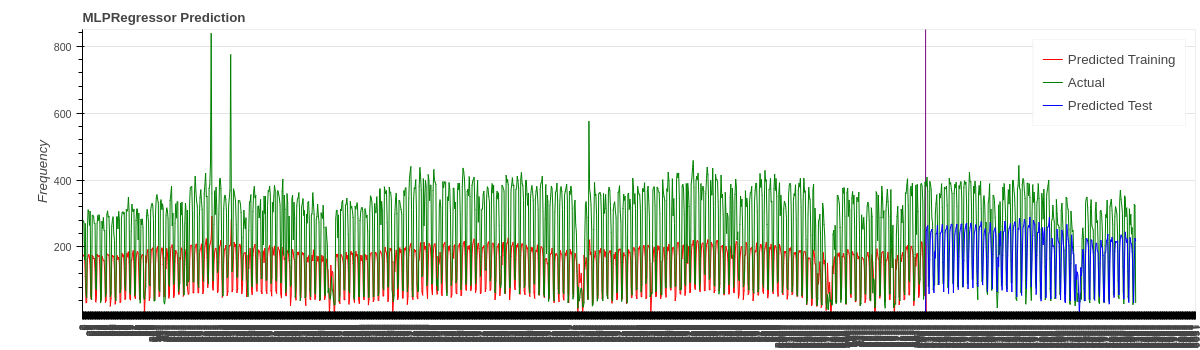
\includegraphics[width=1.4\textwidth]{img/mlpminmax}\label{fig:mlpminmax}
\captionof{figure}{Result of \acs{mlp} with MinMaxScaler}\label{fig:mlpminmax}
\end{figure}
This result shows that the prediction lack accuracy. As we found out this was caused by the MinMaxScaler, since this scaler is very sensitive to the presence of outliers. Therefore we chose another scaler for normalization which is more prone to outliers. In order to find a more suitable scaler, experiments were made with all available scalers of Scikit Learn which met the requirements for the output of the scaling. The best result was achieved by the \emph{QuantileTransformer} with a \acs{rmse} of 57.837, therefore we stuck with this normalization method.
\subsubsection{Feature Evaluation}\label{sec:featureeval}
In order to improve accuracy, further experiments were carried out to evaluate the features. As mentioned earlier the previous predictions were made with a feature matrix of thirteen features. To evaluate which features improve the prediction and which are useless 18 test cases were carried out. Each test case consists of different constellations of features. In the end the different \acs{rmse} values were compared, which can be seen in figure \ref{fig:evalmlp}.
\begin{figure}[H]
\hspace{-1.5cm}
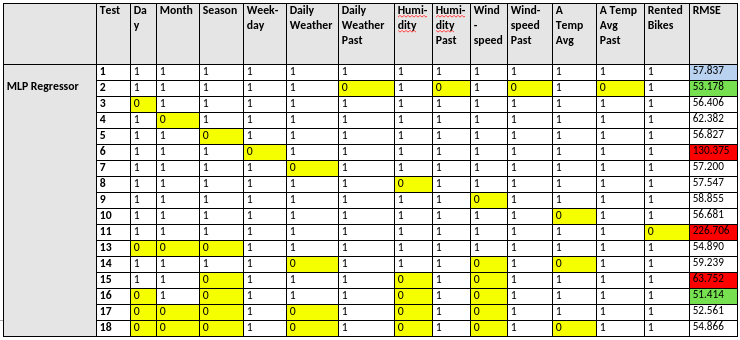
\includegraphics[width=1.2\textwidth]{img/evalmlp}\label{fig:evalmlp}
\captionof{figure}{Feature evaluation test cases}\label{fig:evalmlp}
\end{figure}
Figure \ref{fig:evalmlp} shows beneath the different test cases, included features, those are assigned to \glqq 1\grqq
 and excluded features which are assigned to \glqq 0\grqq. The first \acs{rmse} value, colored in blue depicts the prediction accuracy with all 13 features. The red colored values show the constellations which are significantly worse than the original one and in turn the green values represent the values with an increased accuracy than the original one.
\subsubsection{Result}\label{sec:resultmlp}
This evaluation showed that the features \emph{Weekday} and \emph{Rented Bikes} are the most important ones and in turn the features \emph{Day} and \emph{Season} are less important.
Based on our testing results we recommend to use the following nine features: \emph{Weekday, Month, Past Data, Apparent Temperature (Avg), Daily Weather} and \emph{Rented Bikes}. 
Moreover experiments with scalers showed that the \emph{QuantileTransformer} is more prone to outliers than others and is therefore the scaler of choice.\\
First plots were made with the library \emph{Matplotlib} which turns out to be very restricted and complicated to handle in order to create interactive plots. Therefore we recommend to use \emph{Bokeh} which provides easy to implement interactive plots especially for large data sets.\\
Applying the recommendations regarding scaling and feature evaluation we received a \acs{rmse} value of 51.414 which is the best value achieved during the project phase. The overall result visualized with \emph{Bokeh} can be seen in figure \ref{fig:mlpquantile}.
\begin{figure}[H]
\hspace{-2.8cm}
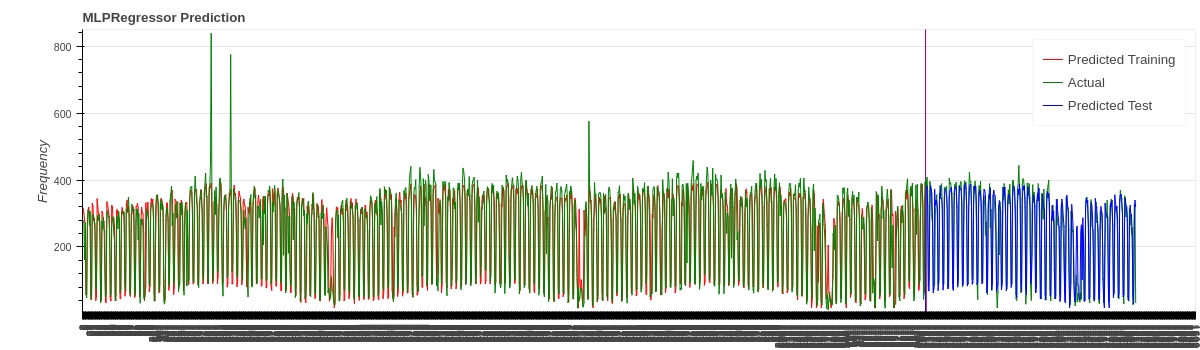
\includegraphics[width=1.4\textwidth]{img/mlpquantile}\label{fig:mlpquantile}
\captionof{figure}{Accuracy with recommended features and scaling by the QuantileTransformer}\label{fig:mlpquantile}
\end{figure}
Compared to figure \ref{fig:mlpminmax} one can see significant improvements in accuracy.\\
This model is based on the most used station, which is King´s Cross with a dataset of 1515 records. In order to confirm this model we applied it to the least used station in Farringdon Street, Holborn as well. The result can be seen in figure  \ref{fig:mlpquantile_least}.
\begin{figure}[H]
\hspace{-2.8cm}
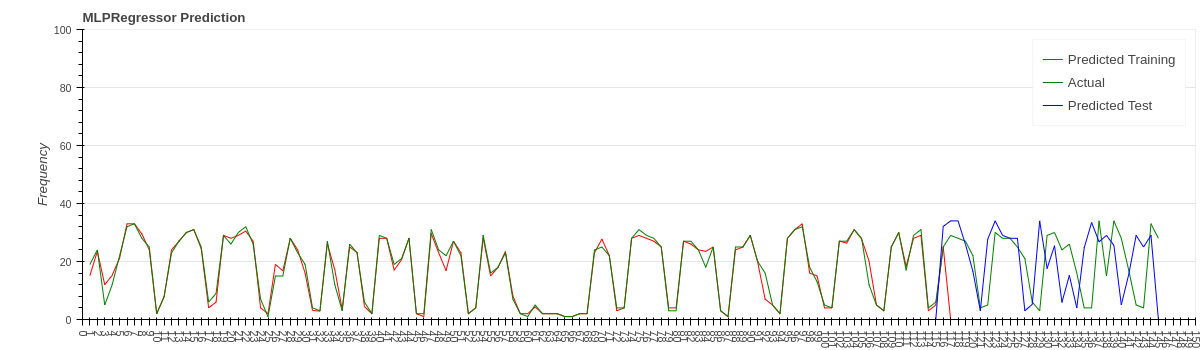
\includegraphics[width=1.4\textwidth]{img/mlpquantile_least}\label{fig:mlpquantile_least}
\captionof{figure}{Accuracy with recommended features and scaling by the QuantileTransformer}\label{fig:mlpquantile_least}
\end{figure}
The accuracy of the prediction of the least used station measures a \acs{rmse} of 9.311. This shows that the model works not only for highly frequented stations but also for stations like Farringdon Street with only 145 records.
\subsection{Modelling (Polynomial Regression)}\label{poly}
Since we don't have a linear relationship between the data, a linear regression will not be helpful.
For example, the regress \glqq Rented Bikes\grqq is not a linear correlation of temperature as even on rainy
days there is slight chance that more people rent a bike than on a sunny day due to a special
holiday. Therefore polynomial regression was a selected machine learning method for the
prediction of rented bikes on a station.\\\\
Polynomial regression belongs to the regression forms \cite{RN9}. In fact, it is just a modified version of a
linear regression. This means the independent variable x and the dependent variable y is modelled
as an nth degress (so-called polynomial) in x \cite{RN9}.\\\\
In a more formal way, the polynomial regression can be expressed as following:
$$Y=\beta_0+\beta_1* x+\beta_2 * x^2 + \beta_3 * x^3 + ... + \beta_n * x^n$$
Where n is the degree of the regression.\\\\
With the scitkit-library in python a data scientist can import the function \glqq PolynomialFeatures\grqq from
\glqq sklearn.preprocessing\grqq which transforms linear data into higher dimensional data. For example
one could apply \glqq poly = PolynomialFeatures(degree = 3)\grqq to get a polynomial
regression in the third dimension. This should improve the accuracy as our underlying data has
no linear relationships but maybe higher dimensional ones. Furthermore, the higher the degree
the better the accuracy should be. Unfortunately the computation time is exponential. A degree of
4 already took several hours to perform and was only slightly better than a regression in the third
dimension.\\\\
The RSME error on a degree of 4 was around 48,4, which is in comparison to the other tested
ones not really bad but maybe also not best one.\\\\
Figure \ref{fig:figure9_polynomial_features} shows the different plots of each feature and the prediction (rented usage). It turns out
that the feature Season, for example, has no German influence on the use of bicycles, whereby
there was apparently an outlier in spring with 800 rented bicycles. It is also becoming apparent
that bicycles are rented more frequently at low wind speeds than at high wind speeds. The average
temperatures between 30 and 70 Fahrenheit are particularly high. Unfortunately, the addition of
the past data has not caused much change in accuracy, as shown in figure \ref{fig:figure9_polynomial_features}.\\\\
Figure \ref{fig:figure10_polynomial_prediction} shows a plot of the tested data (prediction) with the feature \glqq Daily Weather\grqq . The plot looks relatively good, except for a few single outliers at 2 (partly-cloudy-day), the prediction of the
tested data matches the training data.
\begin{figure}[H]
\hspace{-2.8cm}
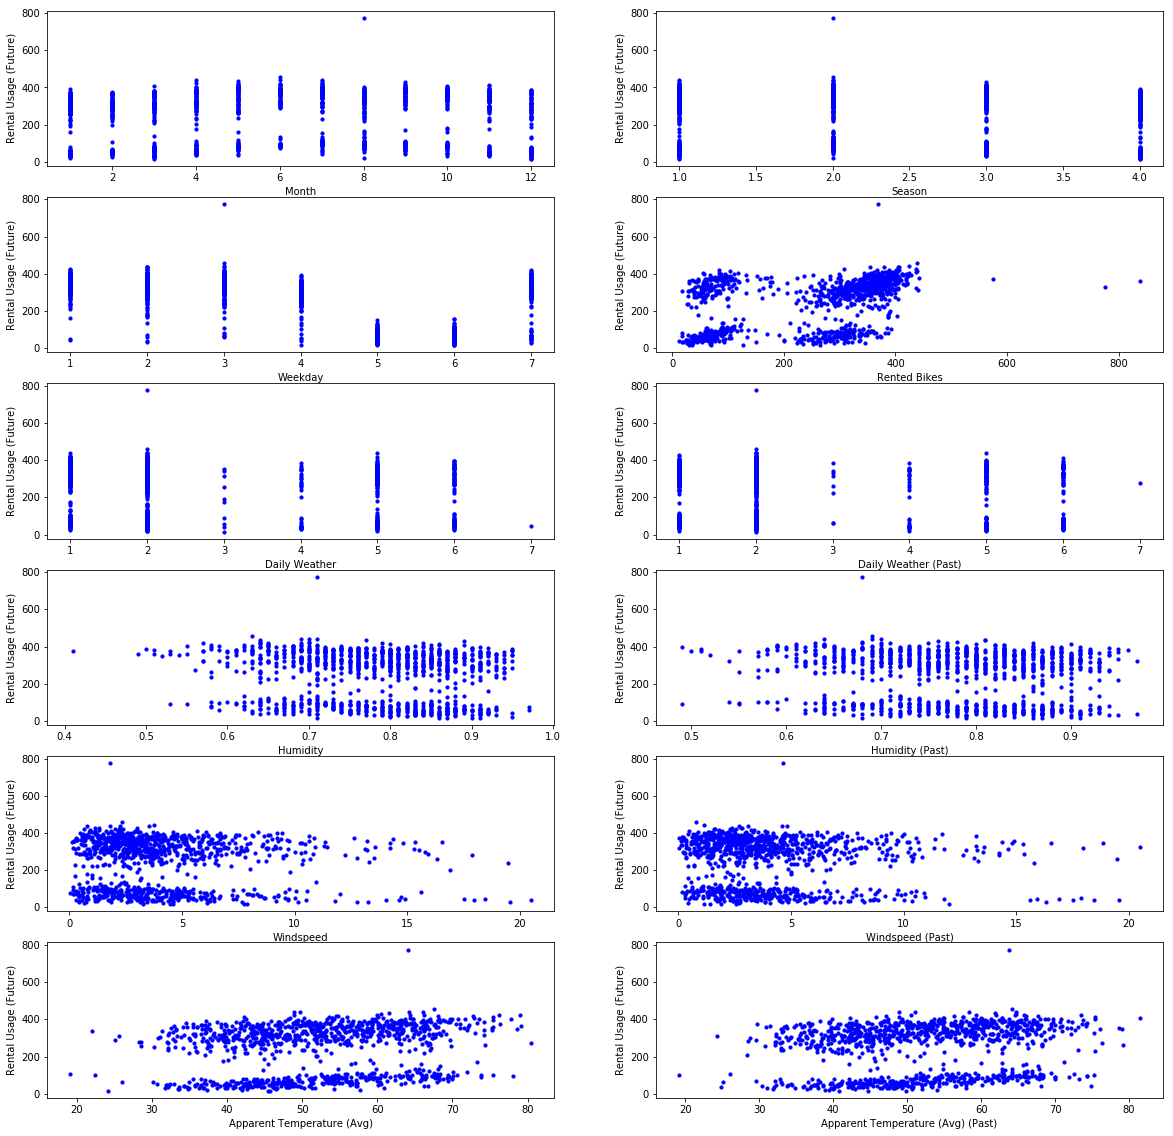
\includegraphics[width=1.4\textwidth]{img/figure9_polynomial_features}\label{fig:figure9_polynomial_features}
\captionof{figure}{Plot of polynomial regression (features)}\label{fig:figure9_polynomial_features}
\end{figure}
\begin{figure}[H]
\hspace{-2.4cm}
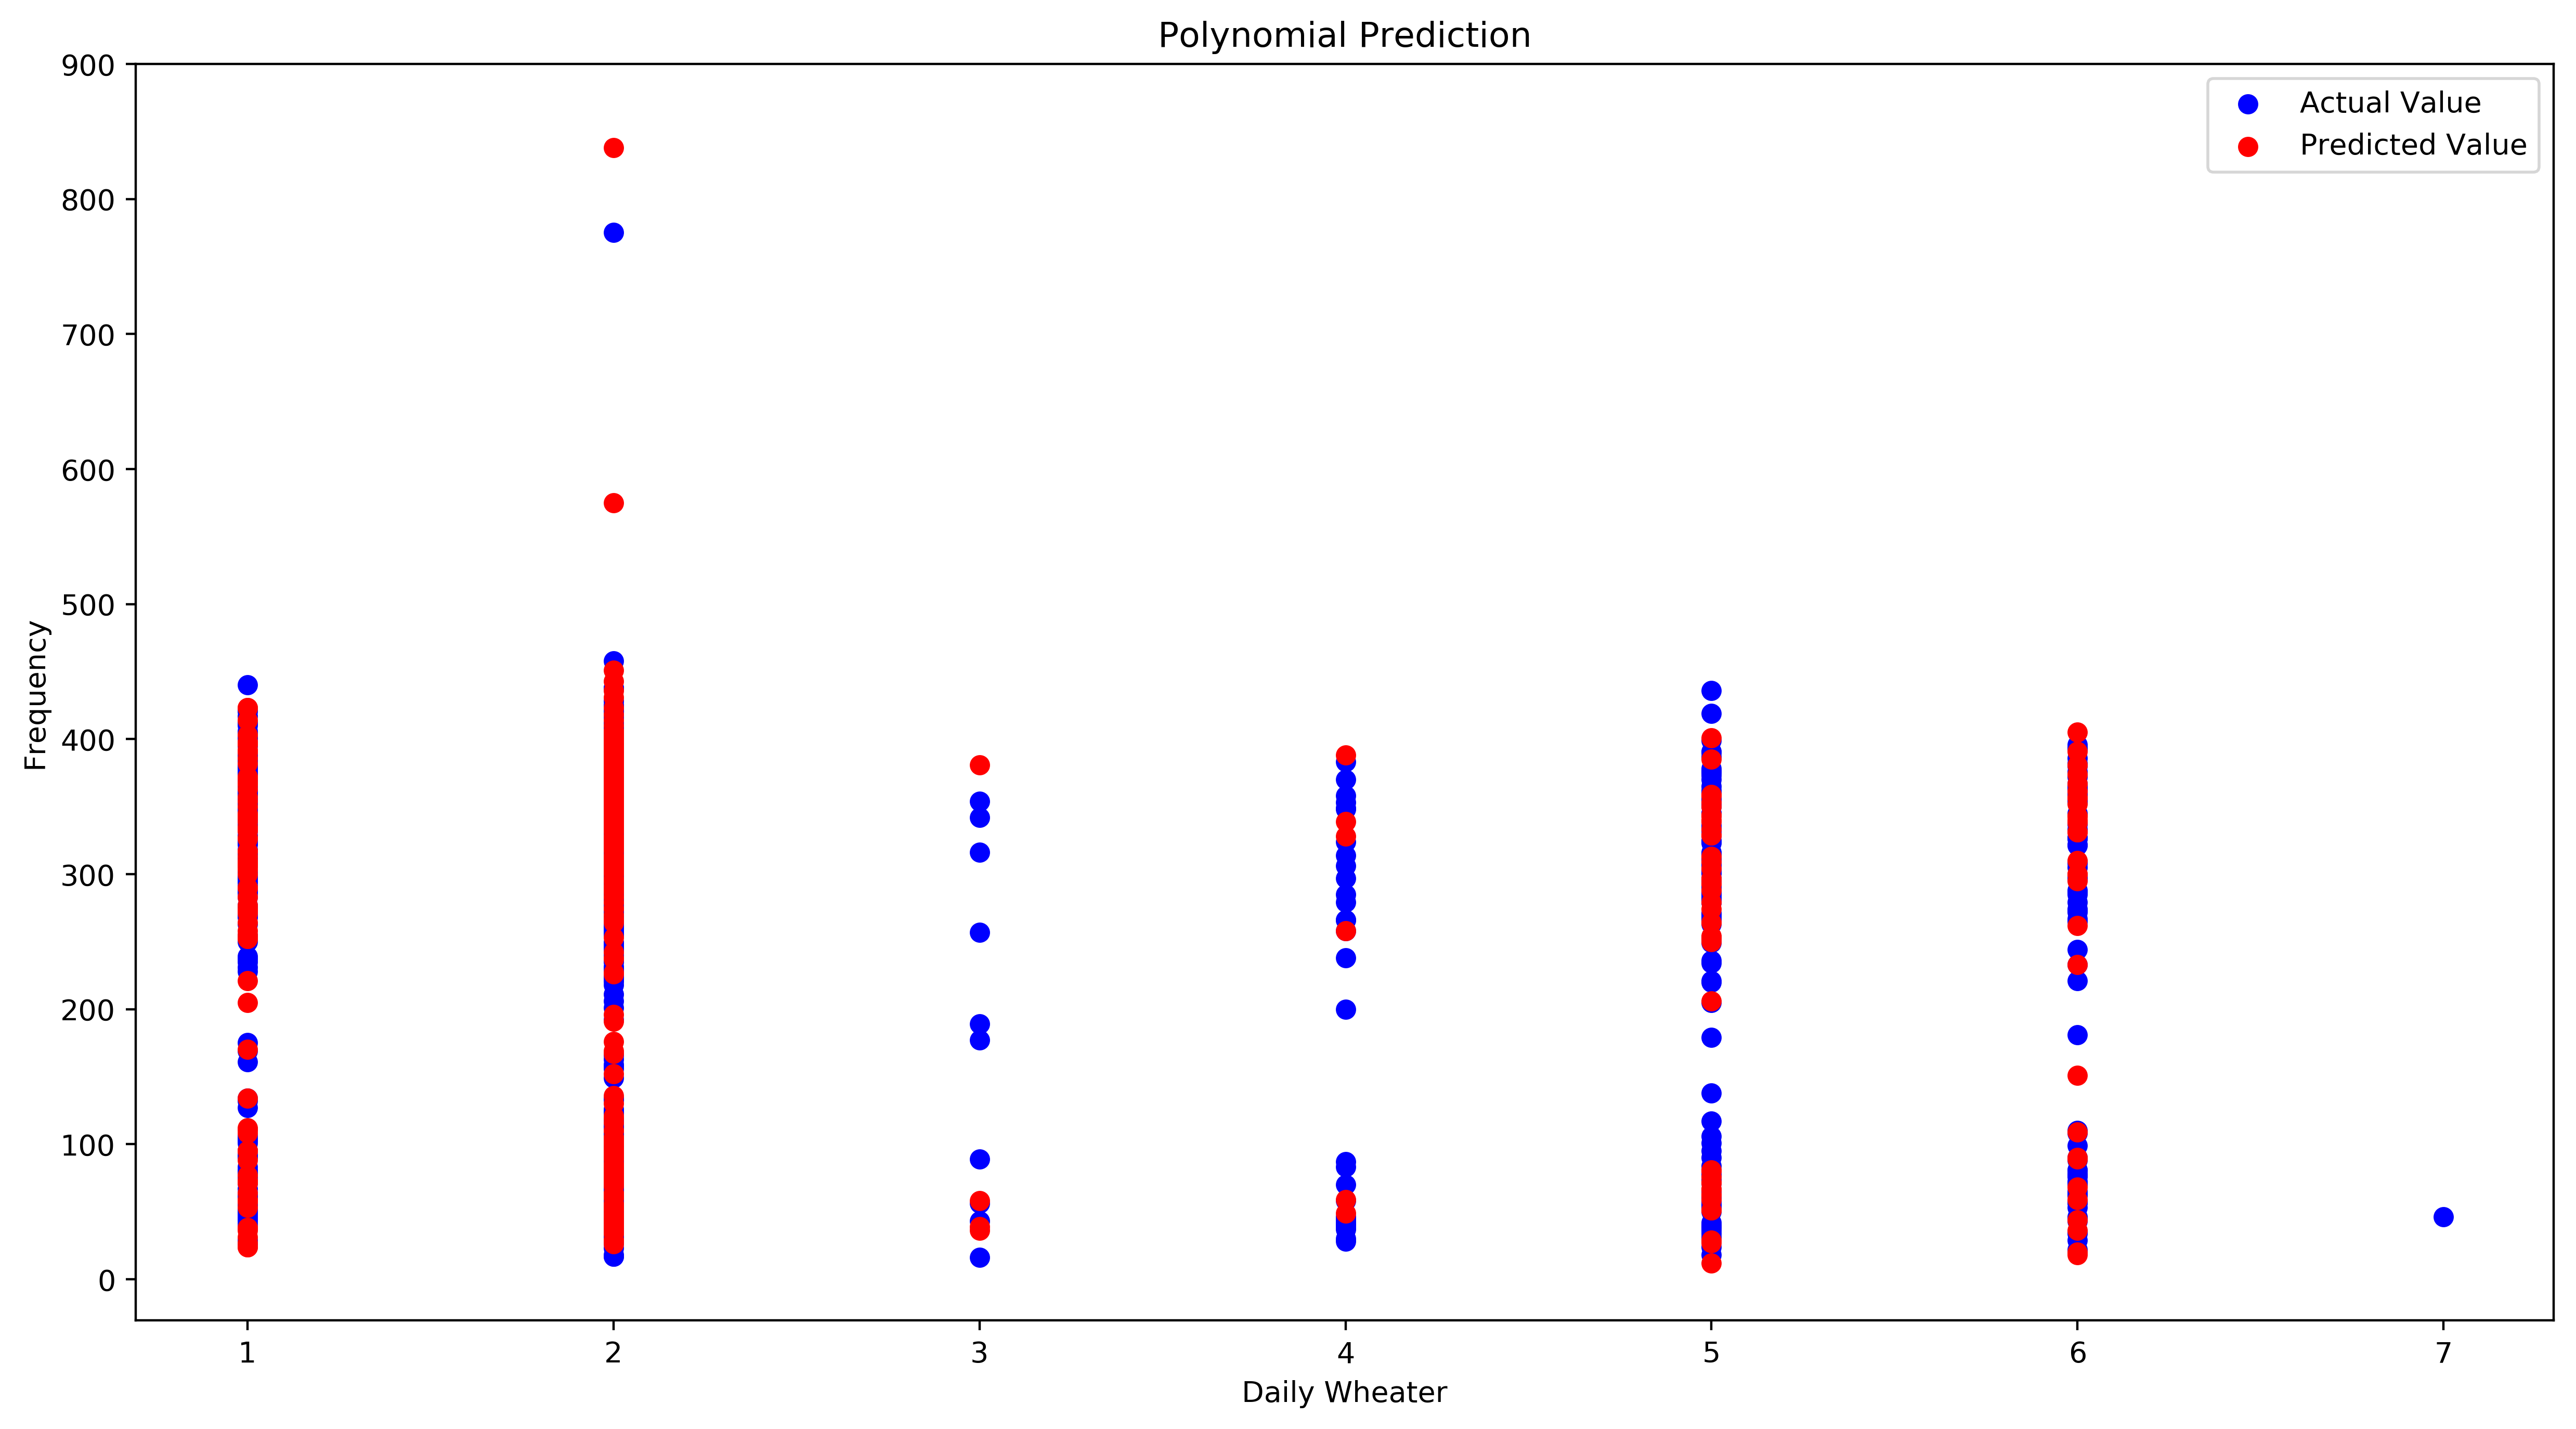
\includegraphics[width=1.3\textwidth]{img/figure10_polynomial_prediction}\label{fig:figure10_polynomial_prediction}
\captionof{figure}{Polynomial Prediction of rental usage on daily weather}\label{fig:figure10_polynomial_prediction}
\end{figure}